\documentclass[final]{beamer}
\usefonttheme{serif}
\mode<presentation>{\usetheme{I6dv}}
\usepackage{amsmath, amsfonts, amssymb, pxfonts, eulervm, xspace, enumerate, hyperref, color, bookmark}
\usepackage{graphicx}
\usepackage[orientation=landscape, size=a0, scale=1.4, debug]{beamerposter}
% \usepackage{natbib}

\usecolortheme{rose}
%\setbeamercolor{background canvas}{bg=magenta!16!yellow!90}

\beamertemplategridbackground[1cm]

%-- Header and footer information ----------------------------------
\newcommand{\footright}{\href{https://github.com/gdmosher/Poster-MSRIP1}{https://github.com/gdmosher/Poster-MSRIP1}}
\newcommand{\footleft}{\href{mailto:thomas.girke@ucr.edu}{Faculty Advisor: Dr. Thomas Girke}}

\def\conference{(MSRIP)}
\title{Reproducible Research and Teaching in the Cloud}
\author{\bf Gordon David Mosher and Thomas Girke} 
\institute{\bf University of California, Riverside - Departments of Statistics and Bioinformatics}
%-------------------------------------------------------------------


%-- Main Document --------------------------------------------------
\usepackage{Sweave}
\begin{document}
\Sconcordance{concordance:SummerBridge3.tex:SummerBridge3.Rnw:%
1 25 1 1 0 5 1 1 34 104 1 1 2 %
14 0 1 1 20 0 1 2 7 1 1 9 52 1 %
1 5 33 1}

\begin{frame}[fragile]
\vspace{-2ex}
\begin{columns}[t]


%-- Column 1 ---------------------------------------------------
\begin{column}{0.31\linewidth}
\begin{minipage}[t][1.000\textheight]{\linewidth} 

%-- Block 1-1
\vspace{0ex}
\begin{block}{Abstract}
\begin{itemize}
\item These days, science is increasingly supported by Data Science. Publishing of scientific data now requires technical skills often outside the realm of the researcher's expertise. This Data Science research project uses nearly twenty computer languages and file formats to move scientific data to the web, yet the end user need only enter a few commands to harness that power.
\item Our research focuses on the automation of documentation tools. Existing documentation tools are connected by custom scripts to create nearly seamless paths for scientific data to reach various output formats. R is a very powerful statistical programming language and RStudio is its user friendly interface, thereby making R's power and interactive data analysis features accessible to scientists in any field. R has the ability to analyze data and create charts and graphs. Further, R will combine these results with markdown text to create complete documents ready for publication. Additional processing can be applied to create novel or specialized output formats.

\end{itemize}
\vspace{0ex}
\end{block}
\vfill

%-- Block 1-2
\begin{block}{** Experienced R Users - Skip to Step 2}
\begin{figure}

\includegraphics[width=0.50\linewidth]{images/RStudio-Logo-Blue-Gradient.png}
\end{figure}
\vspace{0ex}
\vfill
\end{block}
\vfill

%-- Block 3-1
\vspace{0ex}
\begin{block}{Step 1 - Bring your markdown text, LaTeX, and data}
\vspace{0ex}
\begin{figure}
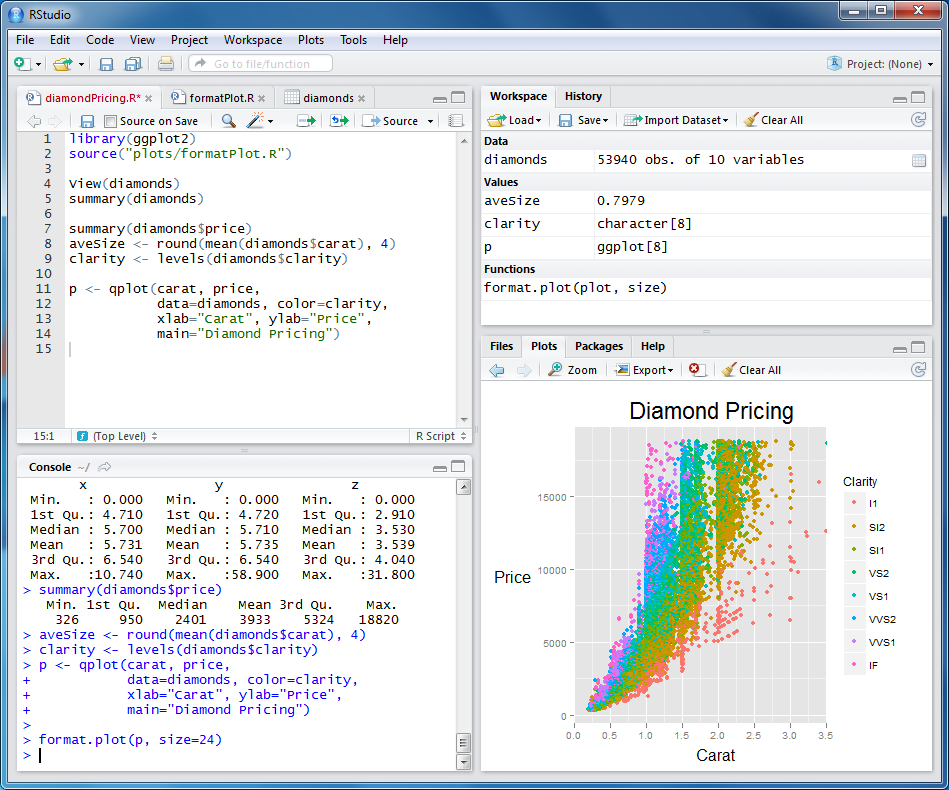
\includegraphics[width=\linewidth]{images/RStudio-Screenshot.png}
\end{figure}

\begin{enumerate}[I.]
\item Least Squares Regression
\vspace{0ex}

Note: Variables are described in the Variable Table handout.
\begin{enumerate}[a.]
\item Model from applied to Training data (\textcolor{blue}{mod1A}) --- Percent voting for Amendment One is modeled using the predictors pct18.24, medinc, pctb, mccain08, evanrate, pctrural, and pctba. 
\item Our OLS model applied to Training data (\textcolor{blue}{mod1B}) --- Percent voting for Amendment One is modeled using the predictors obama08, pctrural, pctw, pctd, pctb, log(pct18.24), log(pctcolenrol), pctfm, log(pctfd), pctown,  medinc, $\text{medinc}^2$, evanrate, $\text{evanrate}^2$, pctfb, $\text{pctfb}^2$, log(pctstud), and log(colden).
\end{enumerate}
\item Cross validated, $K = 10$, and pruned, $n_{\text{leaves}}=4$, regression tree {JF09} (\textcolor{blue}{mod2})
\item Random Forest built from, $n_{\text{trees}} = 5000 $, {AL02} (\textcolor{blue}{mod3})
\end{enumerate}
\vspace{0ex}

\end{block}
\vfill

%-- Block 1-1
\vspace{0ex}
\begin{block}{Abstract}
\begin{itemize}
\item On May 8, 2012, North Carolina voters approved Amendment One.  This poster examines four different models used to predict North Carolina county voting behavior.  
\item The data in this project is split into $K=10$ equal sized parts.  The cross-validation estimate of the prediction error is $$CV(\hat{f\,}\!)=\frac{1}{N}\sum_{i=1}^{N}L(y_i, \hat{f\,}\!^{-K(i)}(x_i)),$$
where $\hat{f\,}\!^{-K}(x)$ denotes the fitted function with the $K$\textsuperscript{th} part of the data removed.
\end{itemize}
\vspace{0ex}
\end{block}
\vfill

\end{minipage}
\end{column}%1

%-- Column 2 ---------------------------------------------------

\begin{column}{0.31\linewidth}
\begin{minipage}[t][.955\textheight]{\linewidth} 

%-- Block 2-1
\vspace{0ex}
\begin{block}{Step 2 - Render to an R Markdown output format}
\vspace{3ex}
\begin{figure}

\includegraphics[width=0.98\linewidth]{images/RMarkdown.png}
\end{figure}

\vspace{0ex}
\begin{figure}

\includegraphics[width=0.98\linewidth]{images/RMarkdownOutput4way.png}
\end{figure}
\vspace{1ex}
\end{block}

\vfill%-- Block 2-1
\vspace{0ex}
\begin{block}{Step 3 - Methods - Apply automation to publication}
\vspace{0ex}
\begin{itemize}
\item The solution to complex publication procedures is to simplify and automate. By realizing the need to streamline the production of quality publications we have discovered several widely accepted documentation tools that can be chained together to simplify the movement of scientific data from the lab to final publication. After having selected these existing tools our method involves the writing of programs that read the coded output of each tool, manipulates it, and then writes out new code that is appropriate input for the next tool in the chain.
\item The goal is to accomplish a task in seconds that previously took hours of skilled human labor. Minimizing error by simplification, and allowing a greater proportion of time and effort to be directed toward creativity and quality.
The result is a finished website, pdf, or journal article in less time and requiring less technical effort.
\item Our methods include support for reproducible research and teaching in the cloud. Reproducible research means that data, functions, code, and text are submitted to the tool and it will evaluate the data and publish the formatted results in the type of report selected. It also includes the ability to verify others work and expand upon it. Teaching in the cloud includes the development and automatic publication of online university courses using the same toolchains.
\end{itemize}
\vspace{2ex}
\end{block}
\vfill

\vfill%-- Block 2-1
\vspace{0ex}
\begin{block}{Methods}
\vspace{0ex}
\begin{Schunk}
\begin{Soutput}
  Sepal.Length Sepal.Width
1          5.1         3.5
2          4.9         3.0
3          4.7         3.2
4          4.6         3.1
5          5.0         3.6
  Petal.Length Petal.Width Species
1          1.4         0.2  setosa
2          1.4         0.2  setosa
3          1.3         0.2  setosa
4          1.5         0.2  setosa
5          1.4         0.2  setosa
\end{Soutput}
\begin{Soutput}
  Sepal.Length    Sepal.Width   
 Min.   :4.300   Min.   :2.000  
 1st Qu.:5.100   1st Qu.:2.800  
 Median :5.800   Median :3.000  
 Mean   :5.843   Mean   :3.057  
 3rd Qu.:6.400   3rd Qu.:3.300  
 Max.   :7.900   Max.   :4.400  
  Petal.Length    Petal.Width   
 Min.   :1.000   Min.   :0.100  
 1st Qu.:1.600   1st Qu.:0.300  
 Median :4.350   Median :1.300  
 Mean   :3.758   Mean   :1.199  
 3rd Qu.:5.100   3rd Qu.:1.800  
 Max.   :6.900   Max.   :2.500  
       Species  
 setosa    :50  
 versicolor:50  
 virginica :50  
\end{Soutput}
\end{Schunk}
\vspace{0ex}
\end{block}
\vfill

%-- Block 2-2
\vspace{0ex}
\begin{block}{King County Real Estate}
\vspace{0ex}
\vspace{0ex}
\end{block}
\vfill

\end{minipage}
\end{column}%2

%-- Column 3 ---------------------------------------------------
\begin{column}{0.31\linewidth}
\begin{minipage}[t][.955\textheight]{\linewidth} 

%-- Block 3-1
\vspace{0ex}
\begin{block}{Conclusion}
\begin{itemize}
\item Simplifying the process of publication for scientists results in more productivity and better quality documents. The publication of scientific data is becoming a Data Science.
\item Finding tools that automate publication are easy to find, but since technology is changing so rapidly, it may be difficult to determine which toolchains to adopt. The tools we currently recommend are free to use and can be installed in Windows, Linux or OS X.
\item All computations and graphs are created with the open source software \texttt{R} \cite{R-base}. This poster was created using a scripted toolchain based on LaTeX, rather than a graphical layout program. 
\end{itemize}
\vspace{0ex}
\end{block}
\vfill

%-- Block 3-1
\vspace{0ex}
\begin{block}{Step 4 - Add to Jekyll Doc Theme and push to GitHub}
\vspace{0ex}
\begin{figure}

\includegraphics[width=0.55\linewidth]{images/jekyll_github.png}
\end{figure}
%--<<fig=TRUE, echo = FALSE, fig.height = 4.5>>=
%--hist(rnorm(1000), col = "green")
%--@
\vspace{0ex}
\vfill
\end{block}
\vfill

%-- Block 3-2
\begin{block}{Results - Reproducible Research in the Cloud}
\begin{figure}
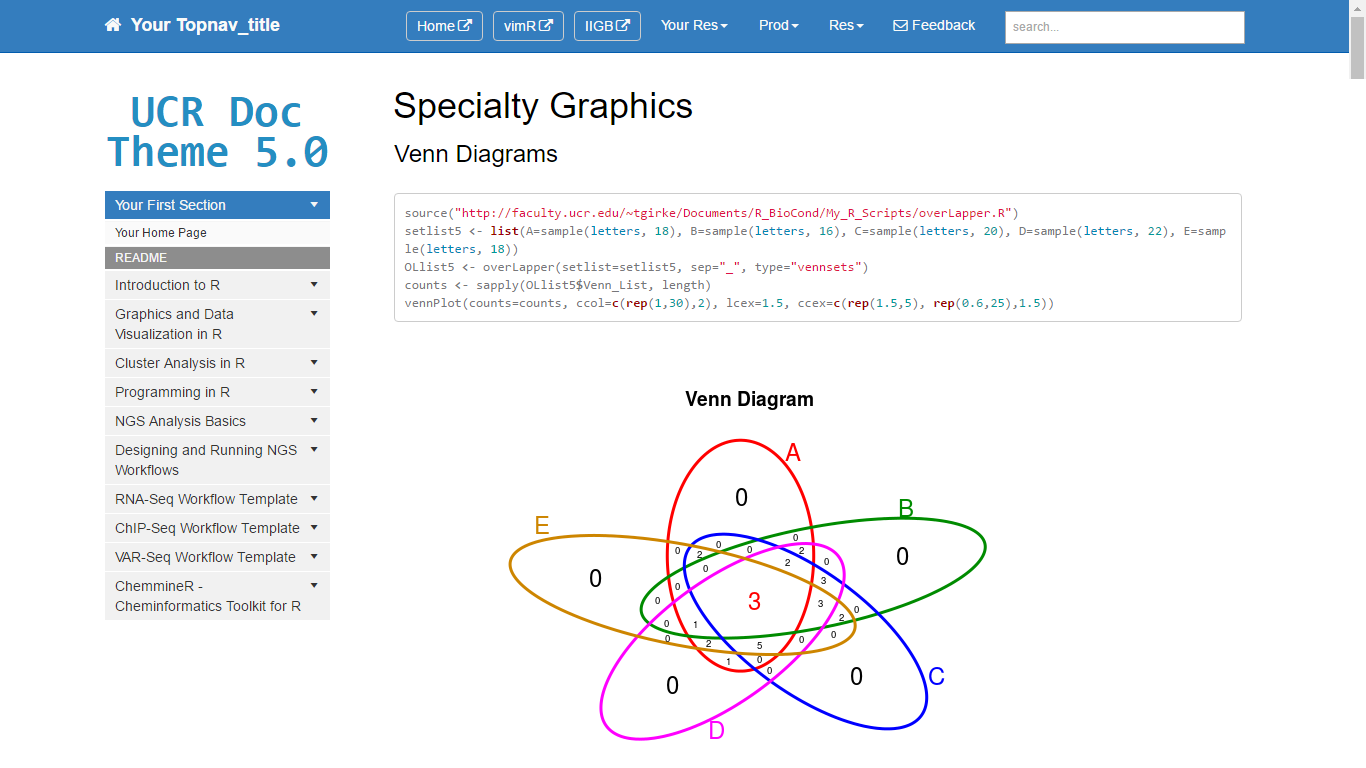
\includegraphics[width=\linewidth]{images/UCRdocTheme.png}
\end{figure}
\vspace{0ex}
\vfill
\end{block}
\vfill

%-- Block 3-4
\begin{block}{References}
\footnotesize
\setbeamertemplate{bibliography item}[text]
\vspace{-1ex}

\bibliographystyle{plain}  % can use plain but comment out natbib at top if using plain
\bibliography{knitr-packages,poster}
\normalsize
\vfill
\end{block} 
\vfill

%-- Block 3-4
\vspace{0ex}
\begin{block}{Acknowledgements}
\vspace{0ex}
\normalsize
\center Mentoring Summer Research Internship Program (MSRIP)
\center CAMP - California Alliance for Minority Participation
\center Sponsored by the National Science Foundation
%--\begin{figure}
%--
\includegraphics[width=0.2\linewidth]{images/NSFhires.jpg}
%--\end{figure}
\vspace{0ex}
\vfill
\end{block} 
\vfill

\end{minipage}
\end{column}%3




\end{columns}
\end{frame}
\end{document}

